\documentclass[First Project.tex]{subfiles}

\begin{document}
\subsection{ Προσπάθεια βελτίωσης της τάξης μίας σελίδας με μία διαφορετική στρατηγική }

Σε αυτή την παράγραφο υλοποιείται ένα υποθετικό σενάριο για το αρχικό δίκτυο μας όπου η ιστοσελίδα 11 θέλει να
βελτιώσει την τάξη της σε σχέση με τον ανταγωνιστή της, την σελίδα 10. Έστω ότι αυτό θέλει να το πετύχει
πείθοντας τις σελίδες 8 και 12 να δείχνουν τη σύνδεση στην 11 με καλύτερο τρόπο και ότι η μοντελοποίηση αυτού 
του σεναρίου γίνεται αντικαθιστώντας το $A_{(8,11)}$ και το $Α_{(12,11)}$ με 3 στον πίνακα γειτνίασης. 

\begin{figure}[h!]
    \centering
    \captionsetup{justification=centering}
    \begin{center}
        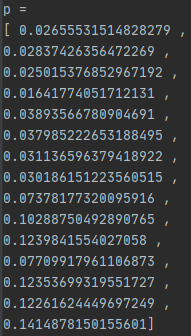
\includegraphics[scale=0.6]{exercise_4_improve_rank_competitor.png}    
        \caption{ Τάξη των σελίδων μετά τις νέες προσθήκες στον πίνακα γειτνίασης του υποθετικού δικτύου μας }
    \end{center}
\end{figure} 

Όπου παρατηρούμε στο \textit{Σχήμα 52} ότι όντως αυτή η στρατηγική δουλεύει και η τάξη της σελίδας 11 αυξήθηκε από $0.10633$ σε 
$0.12398$, ενώ η τάξη του ανταγωνιστή της ( σελίδα 10 ) μειώθηκε από $0.10633$ σε $0.10288$. Ακόμα, αν υπολογίσουμε την πιθανότητα ο χρήστης 
να επιλέξει την σελίδα 11 όταν βρίσκεται στην σελίδα 8 έχουμε 
\begin{equation*}
    p_{\{8->11\}} = \frac{q}{n} + (1-q)\frac{A_{(8,11)}}{n_{8}} = 0.6475
\end{equation*}

ενώ πριν ήταν $0.435$. Αντίστοιχα, για την πιθανότητα ο χρήστης να επιλέξει την σελίδα 11 όταν βρίσκεται στην σελίδα 12 έχουμε
\begin{equation*}
    p_{\{12->11\}} = \frac{q}{n} + (1-q)\frac{A_{(12,11)}}{n_{12}} = 0.6475
\end{equation*}

ενώ πριν ήταν $0.435$. Τέλος, θα μπορούσαμε να σκεφτούμε τον αριθμό 3 στον πίνακα γειτνίασης του δικτύου μας ως ένα βάρος μεταξύ της σύνδεσης
των σελίδων 8 και 12 με την 11 ώστε να δείχνουν με καλύτερο τρόπο, αυτό θα μπορούσε να σημαίνει ότι για παράδειγμα οι σελίδες 8 ή 12 περιέχει 3
συνδέσμους προς την σελίδα 11.
\end{document}